\documentclass[a4paper,12pt]{report}
%%%%%%%%%%%%%%%%%%%%%%%%%%%%%%%%%%%%%%%%%%%%%%%%%%%%%%%%%%%%%%%%%%%%%%%%%%%%%%%%%%%%%%%%%%%%%%%%%%%%%%%%%%%%%%%%%%%%%%%%%%%%%%%%%%%%%%%%%%%%%%%%%%%%%%%%%%%%%%%%%%%%%%%%%%%%%%%%%%%%%%%%%%%%%%%%%%%%%%%%%%%%%%%%%%%%%%%%%%%%%%%%%%%%%%%%%%%%%%%%%%%%%%%%%%%%
\usepackage{eurosym}
\usepackage{vmargin}
\usepackage{amsmath}
\usepackage{graphics}
\usepackage{epsfig}
\usepackage{subfigure}
\usepackage{fancyhdr}
%\usepackage{listings}
\usepackage{framed}
\usepackage{graphicx}

\setcounter{MaxMatrixCols}{10}
%TCIDATA{OutputFilter=LATEX.DLL}
%TCIDATA{Version=5.00.0.2570}
%TCIDATA{<META NAME="SaveForMode" CONTENT="1">}
%TCIDATA{LastRevised=Wednesday, February 23, 2011 13:24:34}
%TCIDATA{<META NAME="GraphicsSave" CONTENT="32">}
%TCIDATA{Language=American English}

\pagestyle{fancy}
\setmarginsrb{20mm}{0mm}{20mm}{25mm}{12mm}{11mm}{0mm}{11mm}
\lhead{MA4128} \rhead{Mr. Kevin O'Brien}
\chead{Advanced Data Modelling}
%\input{tcilatex}


% http://www.norusis.com/pdf/SPC_v13.pdf
\begin{document}


%SESSION 1: Hierarchical Clustering
% Hierarchical clustering - dendrograms
% Divisive vs. agglomerative methods
% Different linkage methods

%SESSION 2: K-means Clustering

\tableofcontents
\newpage

\chapter{Introduction to Cluster Analysis}
\section{Introduction to Cluster Analysis}


%Introduction
\begin{itemize}
	 	\item \textbf{Cluster analysis} is a convenient method for identifying homogenous groups of
	 	objects called clusters. Objects (or cases, observations) in a specific cluster share
	 	many characteristics, but are very dissimilar to objects not belonging to that cluster.
	 	\item  There are three cluster analysis approaches: hierarchical methods,
	 	partitioning methods (more precisely, k-means), and two-step clustering,
	 	which is largely a combination of the first two methods. 
	 	%In the last class we looked as hierarchical clustering analysis.
	 	\item Each of these procedures
	 	follows a different approach to grouping the most similar objects into a cluster and
	 	to determining each object�s cluster membership.

	\item \textbf{\textit{A cluster is a group of relatively homogeneous cases or observations.}}
	\item Cluster analysis is a major technique for classifying a large volumes of information into
	manageable meaningful piles. Cluster analysis is a \textbf{data reduction} tool that creates subgroups that are
	more manageable than individual data items. 
	
	\item The term cluster analysis encompasses a number of different algorithms and methods for grouping objects of similar kind into respective categories.A general question facing researchers in many areas of inquiry is how to organize observed data into meaningful structures, that is, to develop \textbf{\emph{taxonomies}}.
	
	\item \textbf{Cluster analysis} (CA) is an exploratory data analysis tool for organizing observed data into meaningful taxonomies, groups, or
	clusters, based on combinations of independent variables, which maximizes the similarity of cases within
	each cluster while maximizing the dissimilarity between groups that are initially unknown.
	
	\item Both cluster analysis (and later, discriminant
		analysis) are concerned with \textbf{classification}. Each cluster thus describes, in terms of the data collected, the class to
		which its members belong. Items in each cluster are similar in some ways to each other and
		dissimilar to those in other clusters.
		
		\item In this sense, CA creates new groupings without any preconceived notion of what clusters
	may arise, whereas \textit{\textbf{discriminant analysis}} classifies people and items into
	already known groups \\ (\textit{Theory topic for later on : Supervised and Unsupervised Learning}).
	
	\item In other words cluster analysis is an exploratory data analysis tool which aims at sorting different objects into groups in a way that the degree of association between two objects is maximal if they belong to the same group and minimal otherwise. Given the above, cluster analysis can be used to discover structures in data without providing an explanation/interpretation. 
	
	\item \textbf{Important:} Cluster analysis simply discovers structures in data without explaining why they exist. It examines the full complement
	of inter-relationships between variables. Cluster Analysis provides no explanation as to why the clusters exist nor is any
	interpretation made. 
	
	\item However, the latter requires prior knowledge of membership of each cluster in order to classify new cases. In cluster analysis there is no prior knowledge about which elements belong to which clusters. 
	
	\item The grouping 	or clusters are defined through an analysis of the data. Subsequent multivariate analyses
	can be performed on the clusters as groups.

	 	\item Some approaches � most notably hierarchical methods � require us to specify how similar or different objects
	 	are in order to identify different clusters. Most software packages, such as SPSS, calculate a measure
	 	of (dis)similarity by estimating the distance between pairs of objects. Objects with
	 	smaller distances between one another are more similar, whereas objects with larger
	 	distances are more dissimilar.
	
	\item Cluster analysis is a tool of discovery revealing associations and structure in data which, though not previously
	evident, are sensible and useful when discovered. Importantly, CA enables new
	cases to be assigned to classes for identification and diagnostic purposes; or find \textbf{\textit{exemplars}}
	to represent classes.
	
\end{itemize}

\subsection{Types of Cluster Analysis}
There are three main types of cluster analysis.
\begin{itemize}
	\item Hierarchical Clustering Analysis
	\item Non-hierarchical Clustering Analysis (K-means clustering)
	\item Two Step Clustering Analysis
\end{itemize}
\smallskip
\noindent Within hierarchical clustering analysis there are two subcategories: 
\begin{itemize}
	\item Agglomerative (start from n clusters,to get to 1 cluster)
	\item Divisive (start from 1 cluster, to get to $n$ cluster)
\end{itemize}

%------------------------------------------------------------------------------%

\subsection{Steps to conduct a Cluster Analysis}
The process of conducting a hierarchical cluster analysis can be broken into four steps.
\begin{enumerate}
	\item Select a distance measure (e.g. Euclidean Distance).
	\item Select a clustering algorithm (e.g. Ward's Linkage).
	\item Determine the number of clusters (subjective decision based on inspection of the dendrogram).
	\item Validate the analysis
\end{enumerate}

\noindent \textbf{Exercise} Because we usually don't know the number of groups or clusters that will emerge in our sample and because we want an optimum solution, a two-stage sequence of analysis occurs as follows:

\begin{enumerate}
	\item We carry out a hierarchical cluster analysis using \textbf{\textit{Ward' Method}} applying squared
	\textit{\textbf{Euclidean Distance}} as the distance or similarity measure. \item Inspectionf of the dendrogram helps to determine the
	optimum number of clusters we should work with.
	\item The next stage is to rerun the hierarchical cluster analysis with our selected number
	of clusters, which enables us to allocate every case in our sample to a particular
	cluster. \textit{(N.B. SPSS allows for an $n$-cluster solution for hierarchical clsutering.)}
\end{enumerate}

%This sequence and methodology using SPSS will be described in more detail later. There are a variety of clustering procedures of which hierarchical cluster analysis is the major one.

\subsection{Statistical Significance Testing}
\begin{itemize}
	\item Note that the previous discussions refer to clustering algorithms and do not mention anything about statistical significance testing. 
	\item In fact, cluster analysis is not as much a typical statistical test as it is a ``collection" of different algorithms that ``put objects into clusters according to well defined similarity rules."
	
	\item The point here is that, unlike many other statistical procedures, cluster analysis methods are mostly used when we do not have any \textbf{\textit{a priori hypotheses}}, but are still in the exploratory phase of our research. 
	\item In a sense, cluster analysis finds the ``most significant solution possible." Therefore, statistical significance testing is really not appropriate here, even in cases when p-values are reported.
\end{itemize}


\subsection{Dendrograms}

\begin{itemize}
		\item An important question is how to decide on the number of
		clusters to retain from the data. Unfortunately, hierarchical methods provide only
		very limited guidance for making this decision. T
\item The dendrogram is a tree-structured graphical representation, used to visualize of the results of \textbf{\textit{hierarchical cluster analysis}}. 
\item This is a tree-like plot where each step of hierarchical clustering is represented as a joining (or fusion) of two branches of the tree into a single one. 
\item The branches represent clusters obtained on each step of hierarchical clustering. 
\item The result of a clustering is presented either as the \textbf{\textit{distance}} or the similarity between the clustered rows or columns depending on the selected distance measure.
\item T
he only meaningful indicator
relates to the distances at which the objects are combined. Similar to factor
analysis�s scree plot, we can seek a solution in which an additional combination
of clusters or objects would occur at a greatly increased distance. This raises the
issue of what a great distance is, of course. For this purpose, we can make use of the dendrogram.
\end{itemize}
\begin{figure}[h!]
\centering
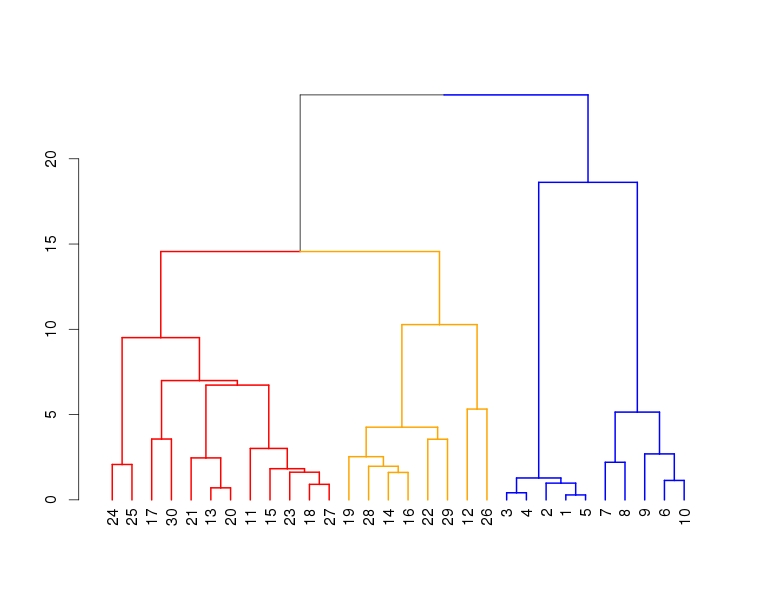
\includegraphics[width=0.7\linewidth]{images/dendrogram1}
\end{figure}
 \begin{itemize}
 	
 	
 	
 	\item A common way to visualize the cluster analysis�s progress is by drawing a
 	dendrogram, which displays the distance level at which there was a combination
 	of objects and clusters.
 	Here is an example of a dendrogram (which corresponds to the example in the next section of material.
 	
 	
 	\begin{figure}[h!]
 		\begin{center}
 			% Requires \usepackage{graphicx}
 			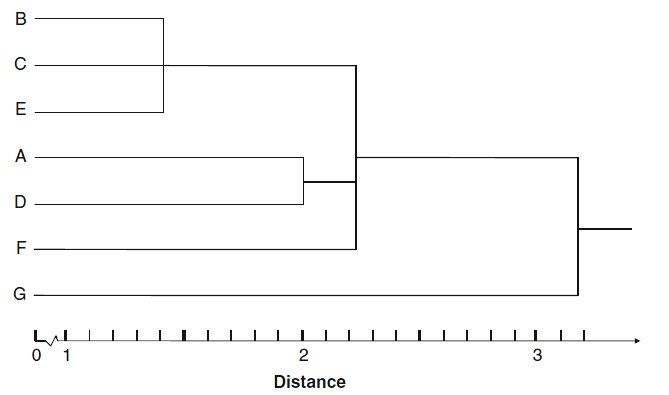
\includegraphics[scale=0.6]{images/Dendrogram.jpg}\\
 		\end{center}
 	\end{figure}
 	
 
 	
 	\item In constructing the dendrogram, SPSS rescales the distances to a range
 	of 0�25; that is, the last merging step to a one-cluster solution takes place at a
 	(rescaled) distance of 25. The rescaling often lengthens the merging steps, thus
 	making breaks occurring at a greatly increased distance level more obvious.
 	Despite this, this distance-based decision rule does not work very well in all
 	cases.
 	
 	It is often difficult to identify where the break actually occurs. This is also
 	the case in our example above. By looking at the dendrogram, we could justify
 	a two-cluster solution ([A,B,C,D,E,F] and [G]), as well as a five-cluster solution
 	([B,C,E], [A], [D], [F], [G]).
 	
 	
 \end{itemize}
%----------------------------------------------------------%
% http://www2.statistics.com/resources/glossary/h/hclusteran.php

% http://mlsc.lboro.ac.uk/resources/statistics/Clusteranalysis.pdf



 \section{Optimal Number of Clusters}
\textit{ (Relevant to all types of clustering analysis)}
 \begin{itemize}

 	\item An important problem in the application of cluster analysis is the decision
 	regarding how many clusters should be derived from the data. This question is
 	explored in the next step of the analysis. 
 	\item A determination may be made by inspection of the dendrogram. Sometimes, however,
 	number of segments that have to be derived from the data will be known in advance.
 	\item
 	By choosing a specific clustering procedure, we determine how clusters are to be
 	formed. (This always involves optimizing some kind of criterion, such as minimizing
 	the within-cluster variance (i.e., the clustering variables� overall variance of
 	objects in a specific cluster), or maximizing the distance between the objects or
 	clusters).
 	\item The procedure could also address the question of how to determine the
 	(dis)similarity between objects in a newly formed cluster and the remaining objects
 	in the dataset.
 \end{itemize}
 \subsection{Types of Hierarchical Clustering}
 \begin{itemize}
 	\item
 	Hierarchical clustering procedures are characterized by the tree-like structure
 	established in the course of the analysis. Most hierarchical techniques fall into a
 	category called \textbf{agglomerative clustering}. In this category, clusters are consecutively
 	formed from objects. Initially, this type of procedure starts with each object
 	representing an individual cluster. 
 	\item These clusters are then sequentially merged
 	according to their similarity. First, the two most similar clusters (i.e., those with
 	the smallest distance between them) are merged to form a new cluster at the bottom
 	of the hierarchy. In the next step, another pair of clusters is merged and linked to a
 	higher level of the hierarchy, and so on. This allows a hierarchy of clusters to be
 	established from the bottom up.
 	\item A cluster hierarchy can also be generated top-down. In \textbf{divisive clustering},
 	all objects are initially merged into a single cluster, which is then gradually split up.
 	\item  \textbf{Important} Divisive procedures are quite rarely used in practice. We therefore
 	concentrate on the agglomerative clustering procedures.
 	\item This means that if an object is assigned
 	to a certain cluster, there is no possibility of reassigning this object to another
 	cluster. This is an important distinction between these types of clustering and
 	partitioning methods such as \textbf{\textit{k-means}}. \medskip
 	\item \textbf{SUMMARY} Agglomerative clustering starts with each case as a separate cluster, i.e. there are as many clusters as cases, and then combines the clusters sequentially, reducing the number of clusters at each step until only one cluster is left.
 \end{itemize}
 \subsection{Things to Watch Out For}
 \begin{itemize}

 	\item
 	In statistics, the occurrence of several variables in a multiple regression model are \textbf{closely correlated} to one another, and carrying the same information, more or less. Multi-collinearity can cause strange results when attempting to study how well individual independent variables contribute to an understanding of the dependent variable, often undermining the analysis.
 	
 	\item In many analysis tasks, the variables under consideration are measured on
 	different scales or levels. This would
 	clearly distort any clustering analysis results. We can resolve this problem by \textbf{\textit{standardizing}}
 	the data prior to the analysis.
 	
 	\item Different standardization methods are available, such as the simple \textbf{\textit{z standardization}},
 	which re-scales each variable to have a mean of 0 and a standard deviation of 1.
 	
 	\item In most situations, however, \textbf{\textit{standardization by range}}(e.g., to a
 	range of 0 to 1 or -1 to 1) is preferable. We recommend standardizing the data
 	in general, even though this procedure can potentially reduce or inflate the variables� influence
 	on the clustering solution.
 	
 \end{itemize}
 
 

\textit{ An understanding of linkage method's other than than Ward method will be expected in the end of year examination.}
 \newpage


\chapter{Fundamentals of Cluster Analysis}

\noindent \textbf{Recall}
\begin{itemize}
\item This is the major statistical method for finding relatively homogeneous clusters of cases based on measured characteristics.

\item The clustering method uses the dissimilarities or distances between objects when forming the clusters. The SPSS programme calculates \textbf{\textit{distances}} between data points in terms of the specified variables.

\item 
A hierarchical tree diagram, called a \textbf{\textit{dendrogram }} on SPSS, can be produced to show the linkage points. The clusters are linked at increasing levels of \textbf{\textit{dissimilarity}}.
\item The actual measure of dissimilarity depends on the measure used.
\end{itemize}



 \section{Clustering Linkage Algorithm : The Fundamentals}
 To better understand how a clustering algorithm works, let�s manually examine
 some of the single linkage procedure�s calculation steps. We start off by looking at
 the initial (Euclidean) distance matrix displayed below. For the time being, we will work on the basis of N\textbf{earest-Neighbour Linkage}.
 
 
 
 \begin{figure}[h!]
 	\begin{center}
 		% Requires \usepackage{graphicx}
 		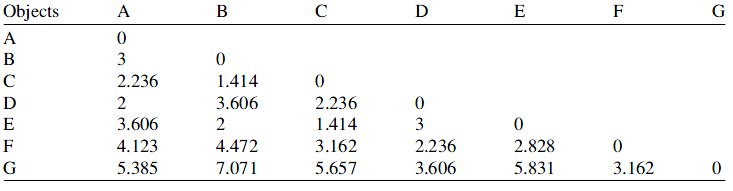
\includegraphics[scale=0.6]{images/DistanceMatrix.jpg}\\
 	\end{center}
 \end{figure}
 
 \begin{itemize}
 	\item In the very first step, the two
 	objects exhibiting the smallest distance (hence the name: nearest neighbour) in the matrix are linked. Note that we
 	always merge those objects with the smallest distance, regardless of the clustering
 	procedure (e.g., single or complete linkage). \\\textit{(N.B. In the following example, ties will be broken at random.)}
 	\item As we can see, this happens to two
 	pairs of objects, namely B and C (\textbf{d(B, C)} = 1.414), as well as C and E (\textbf{d(C, E)} =
 	1.414). \\ In the next step, we will see that it does not make any difference whether we
 	first merge the one or the other, so let�s proceed by forming a new cluster, using
 	objects B and C.
 	\begin{figure}[h!]
 		\begin{center}
 			% Requires \usepackage{graphicx}
 			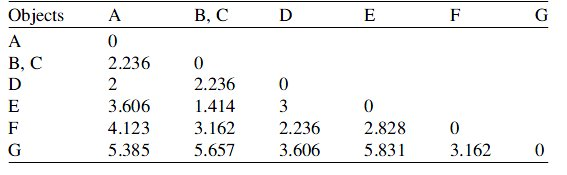
\includegraphics[scale=0.6]{images/DistanceMatrix2.jpg}\\
 		\end{center}
 	\end{figure}
 	\item Having made this decision, we then form a new distance matrix by considering
 	the single linkage decision rule as discussed above. \\ According to this rule, the
 	distance from, for example, object A to the newly formed cluster is the minimum of
 	\textbf{d(A, B)} and \textbf{d(A, C)}. As \textbf{d(A, C)} is smaller than \textbf{d(A, B)}, the distance from A to the
 	newly formed cluster is equal to \textbf{d(A, C)}; that is, 2.236.
 	\item We also compute the
 	distances from cluster [B,C] (clusters are indicated by means of squared brackets)
 	to all other objects (i.e. D, E, F, G) and simply copy the remaining distances � such
 	as \textbf{d(E, F)} � that the previous clustering has not affected.
 	\begin{figure}[h!]
 		\begin{center}
 			% Requires \usepackage{graphicx}
 			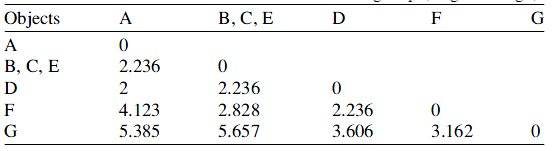
\includegraphics[scale=0.6]{images/DistanceMatrix3.jpg}\\
 		\end{center}
 	\end{figure}
 	\item Continuing the clustering procedure, we simply repeat the last step by merging
 	the objects in the new distance matrix that exhibit the smallest distance (in this case,
 	the newly formed cluster [B, C] and object E) and calculate the distance from this
 	cluster to all other objects.
 	\begin{figure}[h!]
 		\begin{center}
 			% Requires \usepackage{graphicx}
 			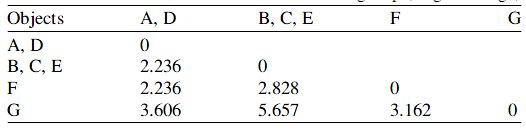
\includegraphics[scale=0.6]{images/DistanceMatrix4.jpg}\\
 		\end{center}
 	\end{figure}
 	\newpage
 	\item We continue in the same fashion until one cluster is left. By following the single linkage procedure, the last steps involve the merger
 	of cluster [A,B,C,D,E,F] and object G at a distance of 3.162.
 	\begin{figure}[h!]
 		\begin{center}
 			% Requires \usepackage{graphicx}
 			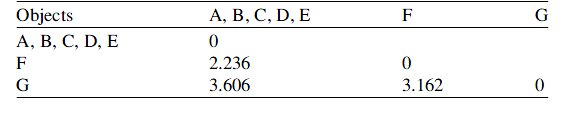
\includegraphics[scale=0.6]{images/DistanceMatrix5.jpg}\\
 		\end{center}
 	\end{figure}
 	\begin{figure}[h!]
 		\begin{center}
 			% Requires \usepackage{graphicx}
 			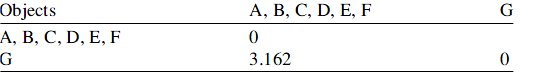
\includegraphics[scale=0.6]{images/DistanceMatrix6.jpg}\\
 		\end{center}
 	\end{figure}
 \end{itemize}
 \newpage
 
 
 
 

\chapter{Linkage}
\section{Linkage Methods for Cluster Analysis}
\begin{itemize}
\item Having selected how we will measure distance, we must now choose the clustering algorithm, i.e. the rules that govern between which points distances are measured to determine cluster membership.
\item  There are many methods available, the criteria used differ and hence
different classifications may be obtained for the same data. This is important since it tells us that, although cluster analysis may provide an objective method for the clustering of cases, there can be subjectivity in the choice of method. 

\item The linkage distances are calculated by SPSS. The goal of the clustering algorithm is to join objects together into successively larger clusters, using some measure of similarity or distance. 
\item SPSS provides seven clustering algorithms, the most commonly used one being  \textbf{\textit{Ward's method}}.
\end{itemize}



\section{Summary of Linkage methods}
\begin{framed}
	\noindent \textbf{Blackboard Examples}
\begin{itemize}
	\item  Single linkage (minimum distance)
	\item  Complete linkage (maximum distance)
	\item  Average linkage
\end{itemize}
\end{framed}

%http://www.rdg.ac.uk/~aes02mm/supermarket.sav
\newpage
\subsection{Ward�s Linkage method (IMPORTANT)}
\begin{itemize}
\item This method is distinct from other methods because it uses an \textbf{\textit{analysis of variance}} approach to evaluate the distances between clusters. In general, this method is very efficient.
\item Cluster membership is assessed by calculating the total sum of squared deviations from the mean of a cluster. The criterion for fusion is that it should produce the smallest possible increase
in the error sum of squares.
\item In this method all possible pairs of clusters are combined and the sum of the squared
distances within each cluster is calculated. This is then summed over all clusters. 
\item The
combination that gives the lowest sum of squares is chosen. This method tends to
produce clusters of approximately equal size, which is not always desirable. It is also
quite sensitive to outliers. 
\item Despite this, it is one of the most popular methods, along
with the average linkage method.
\end{itemize}

\subsection{Ward's method}
\begin{itemize}
	\item A commonly used approach in hierarchical clustering is \textbf{\textit{Ward�s linkage method}}.
	\item This approach does not combine the two most similar objects successively. Instead,
	those objects whose merger optimises the overall \textbf{within-cluster variance} to the
	smallest possible degree, are combined. 
	\item \textbf{IMPORTANT} If you expect somewhat equally sized
	clusters and the data set does not include outliers, you should always use Ward�s
	method. We will use the Ward's linkage method for laboratory exercises.
\end{itemize}
\subsection{Ward�s method}
In this method all possible pairs of clusters are combined and the sum of the squared
distances within each cluster is calculated. This is then summed over all clusters. The
combination that gives the lowest sum of squares is chosen. This method tends to
produce clusters of approximately equal size, which is not always desirable. It is also
quite sensitive to outliers. Despite this, it is one of the most popular methods, along
with the average linkage method.
%\begin{itemize}
%	\item  Compute sum of squared distances within clusters
%	\item  Aggregate clusters with the minimum increase in the
%	overall sum of squares
%\end{itemize}
%\subsubsection{Centroid method}
%The distance between two clusters is defined as the
%difference between the centroids (cluster averages)
%
%
%% http://www.norusis.com/pdf/SPC_v13.pdf
\subsection{Centroid method}
Here the centroid (mean value for each variable) of each cluster is calculated and the
distance between centroids is used. Clusters whose centroids are closest together are
merged. This method is also fairly robust.

\subsection{Linkage Method} 

	

	\begin{itemize}
	\item Other most popular
	agglomerative clustering procedures include the following:
	\begin{description}
		\item[Single linkage (nearest neighbor)]: The distance between two clusters corresponds
		to the shortest distance between any two members in the two clusters.
		\begin{figure}[h!]
			\begin{center}
				% Requires \usepackage{graphicx}
				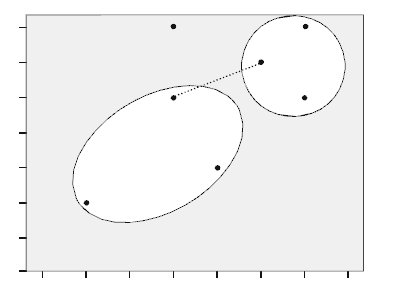
\includegraphics[scale=0.4]{images/Link1.jpg}\\
			\end{center}
		\end{figure}
		\item[Complete linkage (furthest neighbor)]: The oppositional approach to single
		linkage assumes that the distance between two clusters is based on the longest
		distance between any two members in the two clusters.
		\begin{figure}[h!]
			\begin{center}
				% Requires \usepackage{graphicx}
				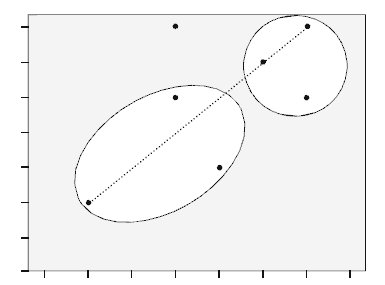
\includegraphics[scale=0.4]{images/Link2.jpg}\\
			\end{center}
		\end{figure}
		\item[Average linkage] : The distance between two clusters is defined as the average
		distance between all pairs of the two clusters� members.
		\begin{figure}[h!]
			\begin{center}
				% Requires \usepackage{graphicx}
				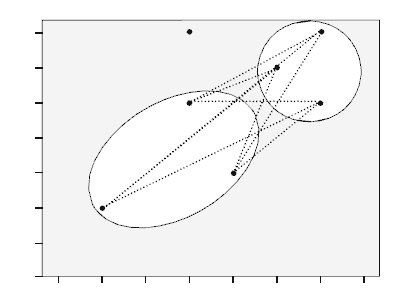
\includegraphics[scale=0.4]{images/Link3.jpg}\\
			\end{center}
		\end{figure}
		\newpage
		\item[Centroid] : In this approach, the geometric center (centroid) of each cluster is
		computed first. The distance between the two clusters equals the distance between
		the two centroids.
		\begin{figure}[h!]
			\begin{center}
				% Requires \usepackage{graphicx}
				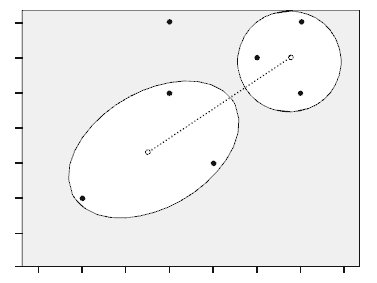
\includegraphics[scale=0.4]{images/Link4.jpg}\\
			\end{center}
		\end{figure}
	\end{description}
	Each of these linkage algorithms can yield totally different results when used on the same data set, as each has its specific properties. As the single linkage algorithm is based on minimum distances, it tends to form one large cluster with the other clusters containing only one or few objects each. We can make use of this \textbf{\textit{chaining effect}} to detect outliers, as these will be merged with the remaining objects � usually at very large distances � in the last steps of the analysis. Generally, single linkage is considered the most versatile algorithm.
	
	Conversely, the complete linkage method is strongly affected by outliers, as it is based on maximum distances. Clusters produced by this method are likely to be rather compact and tightly clustered. The average linkage and centroid algorithms tend to produce clusters with rather low within-cluster variance and similar sizes.
	However, both procedures are affected by outliers, though not as much as complete linkage.
\end{itemize}

\subsection{Nearest neighbour method} 
(Also known as the single linkage method).\\
In this method the distance between two clusters is defined to be the distance between
the two closest members, or neighbours. This method is relatively simple but is often
criticised because it doesn�t take account of cluster structure and can result in a problem
called chaining whereby clusters end up being long and straggly. However, it is better
than the other methods when the natural clusters are not spherical or elliptical in shape.

\subsection{Furthest neighbour method}
\textit{(Also known as the complete linkage method)}.\\
In this case the distance between two clusters is defined to be the maximum distance
between members  i.e. the distance between the two subjects that are furthest apart.
This method tends to produce compact clusters of similar size but, as for the nearest
neighbour method, does not take account of cluster structure. It is also quite sensitive
to outliers.


\subsection{Average (between groups) linkage method }
\textit{(sometimes referred to as Unweighted Pair Group Method with Arithmetic Mean (UPGMA)).}\\
The distance between two clusters is calculated as the average distance between all pairs
of subjects in the two clusters. This is considered to be a fairly robust method.




%\subsection{Ward's Method}
%This method is distinct from other methods because it uses an \textbf{\textit{analysis of variance}} approach to evaluate the distances between clusters. In general, this method is very efficient.
%
%Cluster membership is assessed by calculating the total sum of squared deviations from the mean of a cluster. The criterion for fusion is that it should produce the smallest possible increase
%in the error sum of squares.
%
%
%
%\subsection{Ward's Linkage}
%
%Ward's linkage is a method for hierarchical cluster analysis . The idea has much in common with analysis of variance (ANOVA). The linkage function specifying the distance between two clusters is computed as the increase in the "error sum of squares" (ESS) after fusing two clusters into a single cluster. Ward's Method seeks to choose the successive clustering steps so as to minimize the increase in ESS at each step.





%
%
%
%\subsection{Ward's Linkage}
%
%Ward's linkage is a method for hierarchical cluster analysis . The idea has much in common with analysis of variance (ANOVA). The linkage function specifying the distance between two clusters is computed as the increase in the "error sum of squares" (ESS) after fusing two clusters into a single cluster. Ward's Method seeks to choose the successive clustering steps so as to minimize the increase in ESS at each step.


%
%\subsection{Applications of Cluster Analysis}
%
%In medicine, the clustering of symptoms and diseases leads to taxonomies of illnesses. In the field of business, clusters of consumer segments are often sought for successful marketing strategies. Biologists have to organize the different species of animals before a meaningful description of the differences between animals is possible.

%\subsection{Cluster Analysis as a Statistical Tool}





\chapter{Implementation}
\section{SPSS Implementation and Output}
\begin{itemize}
	\item 
\textbf{Hierarchical Cluster Analysis} is implemented by the \textbf{classify} option on the \textbf{analyse} menu.
Three options shall appear. Select \textbf{Hierarchical}.
\item 
We performed a hierarchical cluster analysis in SPSS, selecting all the variables (except categorical variables) in the \textbf{Variable(s)} box. We can label the cases by a categorical variable. 

\item We shall further requested the Dendrogram in the output. We changed all
variables to z-scores to yield equal metrics and equal weighting, selected the \textbf{Squared Euclidean distance}
(the default) method of determining distance between clusters and the \textbf{Ward's method} for
clustering, and saved a 3-cluster solution as a new variable.
\end{itemize}
\subsection{Proximity matrix}
The output will print distances or similarities computed for any pair of cases. We will not be covering this in detail.

\subsection{Cluster Membership}
\begin{itemize}
\item This box allows you to specify a set number of clusters. 
\item If you have a
hypothesis about how many clusters there are, you can specify a set number of clusters, or
create a number of clusters within a range.
\end{itemize}


\subsection{Icicle Plot} 
\begin{itemize}
\item Default choice by SPSS. 
\item Icicle plots visually represent information on the agglomeration
schedule. You can select that all clusters are included in the icicle plot, or restrict it to a range of
clusters. 
\item Also, you can read the plot from bottom up (vertical orientation) or from left to right
(horizontal orientation).
\end{itemize}


\subsection{SPSS Agglomeration Schedule}
The procedure followed by cluster analysis at Stage 1 is to cluster the two cases that have the smallest
squared Euclidean distance between them. Then SPSS will recompute the distance measures between all
single cases and clusters (there is only one cluster of two cases after the first step). Next, the 2 cases (or
clusters) with the smallest distance will be combined, yielding either 2 clusters of 2 cases (with 17 cases
unclustered) or one cluster of 3 (with 18 cases unclustered).  This process continues until all cases are clustered into a single group.
\begin{center}
\begin{figure}[h!]
	% Requires \usepackage{graphicx}
	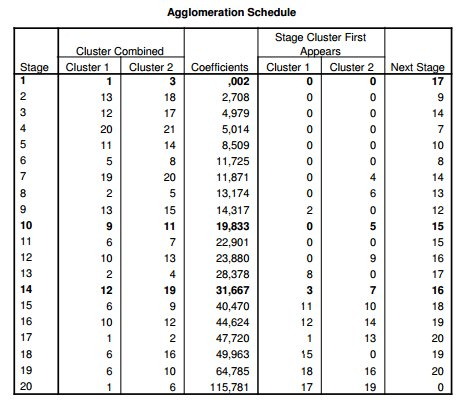
\includegraphics[scale=0.7]{images/AggloSc}\\
	\caption{SPSS Agglomeration Schedule}
\end{figure}
\end{center}



For the sake of clarify, we will explain Stages 1, 10, and 14.


\subsubsection*{Stage 1}
\begin{itemize}
\item At Stage 1, Case 1 is clustered with Case 3. The squared Euclidean distance between these two cases is
.002. \item Neither variable has been previously clustered (the two zeros under Cluster 1 and Cluster 2), and the
next stage (when the cluster containing Case 1 combines with another case) is Stage 17. 
\item (Note that at Stage
17, Case 2 joins the Case-1 cluster.)
\end{itemize}


\subsubsection*{Stage 10}
\begin{itemize}
\item At Stage 10, Case 9 joins the Case-11 cluster (Case 11 was previously clustered with Case 14 back in Stage
5, thus creating a cluster of 3 cases: Cases 9, 11, and 14). \item The squared Euclidean distance between Case 9
and Case-11 cluster is 19.833. Case 9 has not been previously clustered (the zero under Cluster 1), and
Case 11 was previously clustered at Stage 5. \item The next stage (when the cluster containing Case 9 clusters) is
Stage 15 (when it combines with the Case-6 cluster).
\end{itemize}


\subsubsection*{Stage 14}
\begin{itemize}
\item At Stage 14, the clusters containing Cases 12 and 19 are joined, Case 12 has been previously clustered with
Case 17, and Case 19 had been previously clustered with Cases 20 and 21, thus forming a cluster of 5 cases
(Cases 12, 17, 19, 20, 21). 
\item The squared Euclidean distance between the two joined clusters is 31.667. Case
12 was previously joined at Stage 3 with Case 17. Case 19 was previously joined at Stage 7 with the Case-
20 cluster. 
\item The next stage when the Case-12 cluster will combine with another case/cluster is Stage 16
(when it joins with the Case-10 cluster).
\end{itemize}


\begin{figure}
  % Requires \usepackage{graphicx}
  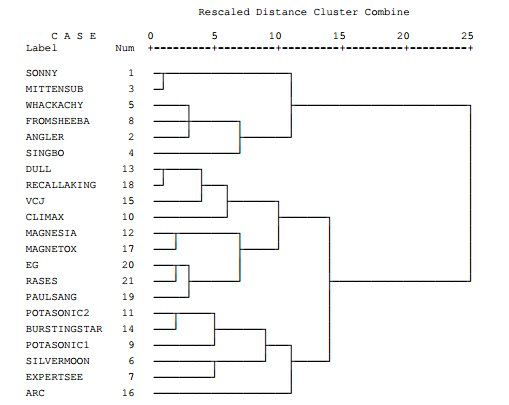
\includegraphics[scale=0.7]{images/Dendro}\\
  \caption{Corresponding Dendrogram}
\end{figure}

The branching-type nature of the Dendrogram allows you to trace backward or forward to any individual
case or cluster at any level. It, in addition, gives an idea of how great the distance was between cases or
groups that are clustered in a particular step, using a 0 to 25 scale along the top of the chart. While it is
difficult to interpret distance in the early clustering phases (the extreme left of the graph), as you move to
the right relative distance become more apparent. The bigger the distances before two clusters are joined,
the bigger the differences in these clusters. To find a membership of a particular cluster simply trace
backwards down the branches to the name.

\newpage


\chapter{Kmeans Clustering}
\section{Non-Hierarchical Clustering (k-Means)}
This method of clustering is very different from the hierarchical clustering and Ward method, which are applied when there is no prior knowledge of how many clusters there may be or what they are characterized by. The k-means clustering approach is used when you already have hypotheses concerning the number of clusters in your cases or variables. For example, you may want to specify exactly three clusters that are to be as distinct as possible.

This is the type of research question that can be addressed by the k-means clustering algorithm. In general, the k-means method will produce the exact k different clusters demanded of greatest possible distinction. Very often, both the hierarchical and the k-means techniques are used successively.
\begin{itemize}
\item Ward's method is used to get some sense of the possible number of clusters and the way they merge as seen from the dendrogram.
\item Then the clustering is rerun with only a chosen optimum number in which to place all
the cases (i.e. k means clustering).
\end{itemize}

\subsection{Procedure for k-means}
In these methods the desired number of clusters is specified in advance and the `best' solution
is chosen. The steps in such a method are as follows:
\begin{itemize}
\item[1] Choose initial cluster centres (essentially this is a set of observations that are far apart
� each subject forms a cluster of one and its centre is the value of the variables for
that subject).
\item[2] Assign each subject to its `nearest' cluster, defined in terms of the distance to the
centroid.
\item[3] Find the centroids of the clusters that have been formed
\item[4] Re-calculate the distance from each subject to each centroid and move observations that
are not in the cluster that they are closest to.
\item[5] Continue until the centroids remain relatively stable.
\end{itemize}

\subsection{Considerations for Usage of k-means}
Non-hierarchical cluster analysis tends to be used when large data sets are involved. It is
sometimes preferred because it allows subjects to move from one cluster to another (this is
not possible in hierarchical cluster analysis where a subject, once assigned, cannot move to a
different cluster). Two disadvantages of non-hierarchical cluster analysis are: 
\begin{itemize}
\item[1] It is often
diffcult to know how many clusters you are likely to have and therefore the analysis may have
to be repeated several times 
\item[2] It can be very sensitive to the choice of initial cluster centres. Again, it may be worth trying different ones to see what impact this has.
\end{itemize}


 \section{K-Means Clustering}
 \begin{itemize}
 	\item Hierarchical clustering requires a distance or similarity matrix between all pairs of cases. That's an extremely large matrix if you have tens of thousands of cases in your data file.
 	
 	\item A clustering method that doesn't require computation of all possible distances is k-means clustering. It differs from hierarchical clustering in several ways. You have to know in advance the number of clusters you want. You can't get solutions for a range of cluster numbers unless you rerun the analysis for each different number of clusters.
 	
 	\item The algorithm repeatedly reassigns cases to clusters, so the same case can move from cluster to cluster during the analysis. In agglomerative hierarchical clustering, on the other hand, cases are added only to existing clusters. They are forever captive in their cluster, with a widening circle of ``neighbours".
 	
 	\item The algorithm is called \textbf{k-means}, where \textbf{k} is the number of clusters you want, since a case is assigned to the cluster for which its distance to the cluster mean is the smallest.
 	
 	\item The k-means algorithm follows an entirely different concept than the hierarchical methods
 	discussed before. This algorithm is not based on distance measures such as
 	Euclidean distance or city-block distance, but uses the \textbf{\textit{within-cluster variation}} as a measure to form homogenous clusters. Specifically, the procedure aims at segmenting
 	the data in such away that the within-cluster variation isminimized.Consequently,we
 	do not need to decide on a distance measure in the first step of the analysis.
 	
 	\item The action in the algorithm centers around finding the k-means. You start out with an initial set of means and classify cases based on their distances to the centers.
 	
 	\item Next, you compute the cluster means again, using the cases that are assigned to the cluster; then, you reclassify all cases based on the new set of means. You keep repeating this step until cluster means don't change much between successive steps.
 	
 	\item Finally, you calculate the means of the clusters once again and assign the cases to their permanent clusters.
 \end{itemize}
 %------------------------------------------------------------------%
 \subsection{Initial Cluster Centres}
\begin{itemize}
\item The first step in k-means clustering is finding the k centres. This is done iteratively. You start with an initial set of centres and then modify them until the change between two iterations is small enough.
 
\item If you have good guesses for the centres, you can use those
 as initial starting points; otherwise, you can let SPSS find k cases that are well separated and use these values as initial cluster centers. (i.e. The clustering process starts by randomly assigning objects to a number of
 clusters).
 
 
 
\item  K-means clustering is very sensitive to outliers, since they will usually be selected as initial cluster centers. This will result in outliers forming clusters with small numbers of cases. Before you start a cluster analysis, screen the data for outliers and remove them from the initial analysis. The solution may also depend on the order of the cases in the data.
 
\item  After the initial cluster centers have been selected, each case is assigned to the closest
 cluster, based on its distance from the cluster centers. After all of the cases have been
 assigned to clusters, the cluster centers are recomputed, based on all of the cases in the
 cluster.
 
\item  The cases are then successively reassigned to other clusters to minimize the within-cluster variation, which is basically the (squared) distance from each observation to the center of the associated cluster. If the reallocation of an case to another cluster decreases the within-cluster variation, this case is reassigned
 to that cluster.
 
\item  Case assignment is done again, using these updated cluster centers. You keep
 assigning cases and recomputing the cluster centers until no cluster center changes
 appreciably or the maximum number of iterations (10 by default) is reached.
\end{itemize}
 \newpage
 \subsection{Demonstration of k-means}
 In this example, two cluster centers are randomly
 initiated, which CC1 (first cluster) and CC2 (second cluster).
 \begin{figure}[h!]
 	\begin{center}
 		% Requires \usepackage{graphicx}
 		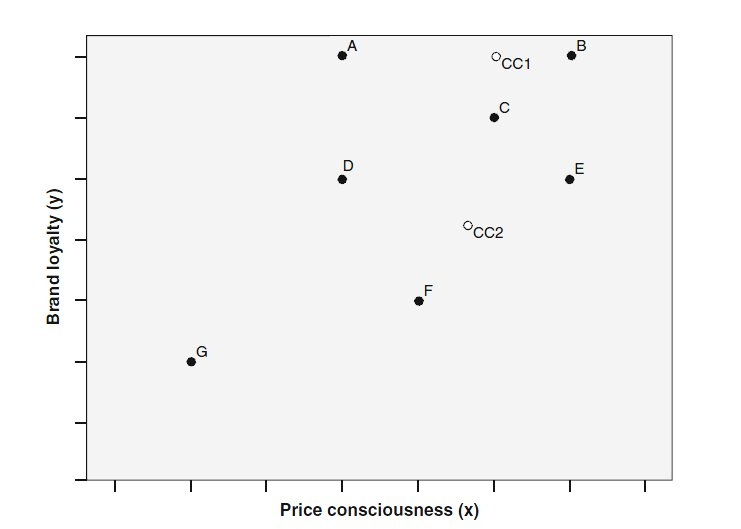
\includegraphics[scale=0.4]{images/kmeans1.jpg}\\
 	\end{center}
 \end{figure}
 \begin{figure}[h!]
 	\begin{center}
 		% Requires \usepackage{graphicx}
 		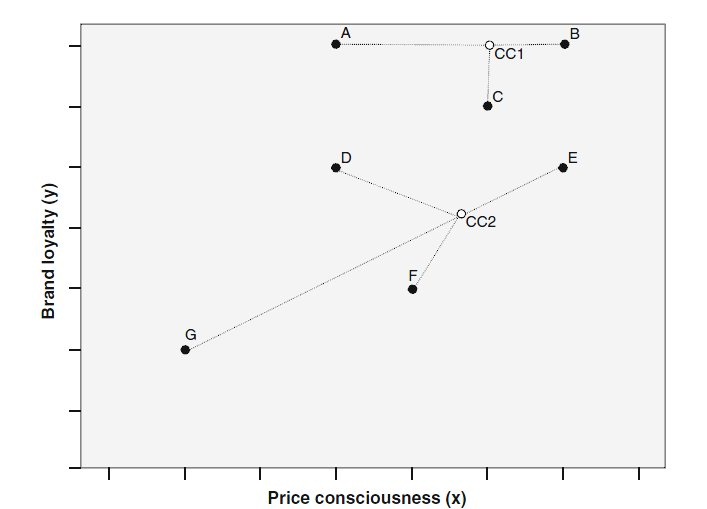
\includegraphics[scale=0.4]{images/kmeans2.jpg}\\
 	\end{center}
 \end{figure}
 Euclidean distances are computed from the cluster
 centers to every single object. Each object is then assigned to the cluster center with
 the shortest distance to it.
 
 In this example, objects A, B, and C are
 assigned to the first cluster, whereas objects D, E, F, and G are assigned to the
 second. We now have our initial partitioning of the objects into two clusters.
 Based on this initial partition, each cluster�s geometric center (i.e., its centroid)
 is computed (third step). This is done by computing the mean values of the objects
 contained in the cluster (e.g., A, B, C in the first cluster) regarding each of the variables
 (in this example: price consciousness and brand loyalty).
 \begin{figure}[h!]
 	\begin{center}
 		% Requires \usepackage{graphicx}
 		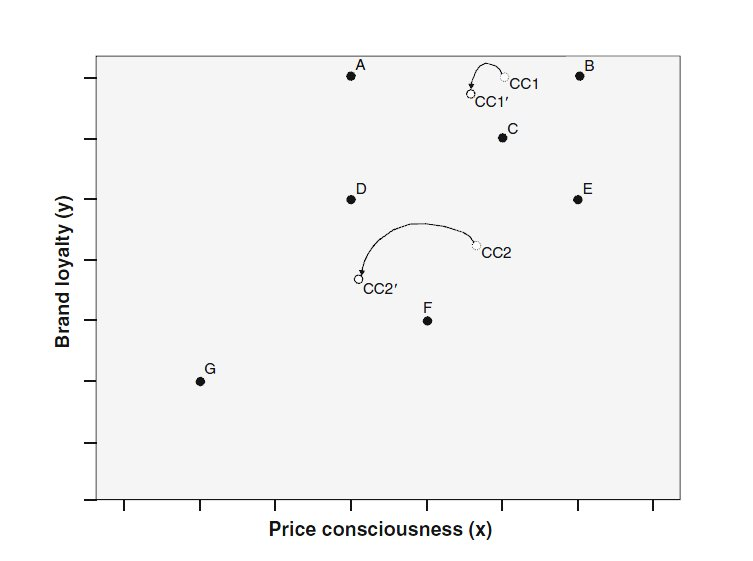
\includegraphics[scale=0.6]{images/kmeans3.jpg}\\
 	\end{center}
 \end{figure}
 \begin{figure}[h!]
\begin{center}
 		% Requires \usepackage{graphicx}
 		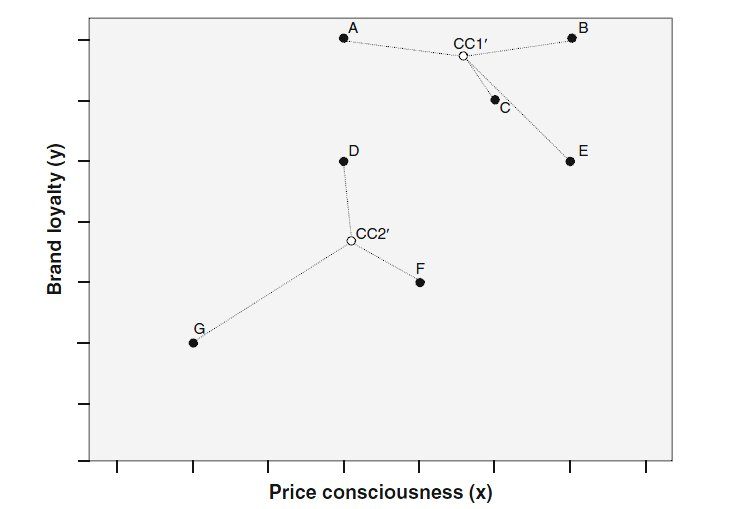
\includegraphics[scale=0.6]{images/kmeans4.jpg}\\
 	\end{center}
 \end{figure}
 Both clusters�centers now shift into new positions (CC1� for the first and CC2� for the second cluster).
 In the fourth step, the distances from each object to the newly located cluster
 centers are computed and objects are again assigned to a certain cluster on the basis
 of their minimum distance to other cluster centers (CC1� and CC2�).
 
 Since the cluster centers� position changed with respect to the initial situation in the first step,
 this could lead to a different cluster solution. This is also true of our example, as
 object E is now � unlike in the initial partition � closer to the first cluster center
 (CC1�) than to the second (CC2�). Consequently, this object is now assigned to the
 first cluster.
 The k-means procedure now repeats the third step and
 re-computes the cluster centers of the newly formed clusters, and so on.
 In other words, steps 3 and 4 are repeated until a predetermined number of iterations are
 reached, or convergence is achieved (i.e., there is no change in the cluster affiliations).
 
\subsection{Optimal Number of Clusters}
One of the biggest problems with cluster analysis is identifying the optimum number of
clusters. As the joining process continues, increasingly dissimilar clusters must be joined. i.e. the classification becomes increasingly artificial. Deciding upon the optimum number
of clusters is largely subjective, although looking at a dendrogram would help.


 \subsection{Performance of k-means clustering}
 \begin{itemize}
\item  Generally, k-means is superior to hierarchical methods as it is less affected by
 outliers and the presence of irrelevant clustering variables. Furthermore, k-means
 can be applied to very large data sets, as the procedure is less computationally
 demanding than hierarchical methods. 
 \item In fact, we suggest definitely using k-means
 for sample sizes above 500, especially if many clustering variables are used. From
 a strictly statistical viewpoint, k-means should only be used on interval or ratio-scaled
 data as the procedure relies on Euclidean distances. However, the procedure is
 routinely used on ordinal data as well, even though there might be some distortions.
 \item 
 One problem associated with the application of k-means relates to the fact that
 the researcher has to pre-specify the number of clusters to retain from the data. This
 makes k-means less attractive to some and still hinders its routine application in
 practice.
 
 \end{itemize}



%------------------------------------------------------------------%

\end{document}